This chapter covers the implementation of the text-aware process prediction model presented in the previous chapter.
In the first section the underlying technology is depicted, whereas in the second section the architecture of the implementation is described.

\section{Technology Stack}

The implementation is realized using Python 3.6 only.

\begin{table}[!htbp]
	\begin{tabularx}{\textwidth}{l p{4.5cm} p{6.6cm} }
		\toprule
		\textbf{Package} & \textbf{Developer(s)} & \textbf{Purpose}  \\
		\midrule
		PM4Py \cite{DBLP:journals/corr/abs-1905-06169}   &  Fraunhofer Institute for Applied Information Technology &  Event log parsing and handling\\
		Tensorflow \cite{DBLP:journals/corr/AbadiABBCCCDDDG16} &  Google Brain Team et al.& Construction and training of LSTM model \\
		Scikit-learn \cite{DBLP:journals/jmlr/PedregosaVGMTGBPWDVPCBPD11}& Cournapeau et al.& Bag of words and bag of n-gram tf-idf encoding \\
		Gensim \cite{rehurek_lrec} & Řehůřek et al. & Latent Dirichlet Allocation and Paragraph Vector encoding \\
		NTLK \cite{DBLP:books/daglib/0022921} & Bird et al. & Text prepossessing\\
		 \bottomrule
	\end{tabularx}
	\caption[List of Python packages used for implementation]{List of Python packages used for implementation.}
	\label{tab:packages}
\end{table}

\section{Model Implementation}

\begin{figure}[htbp!]
	\centering
	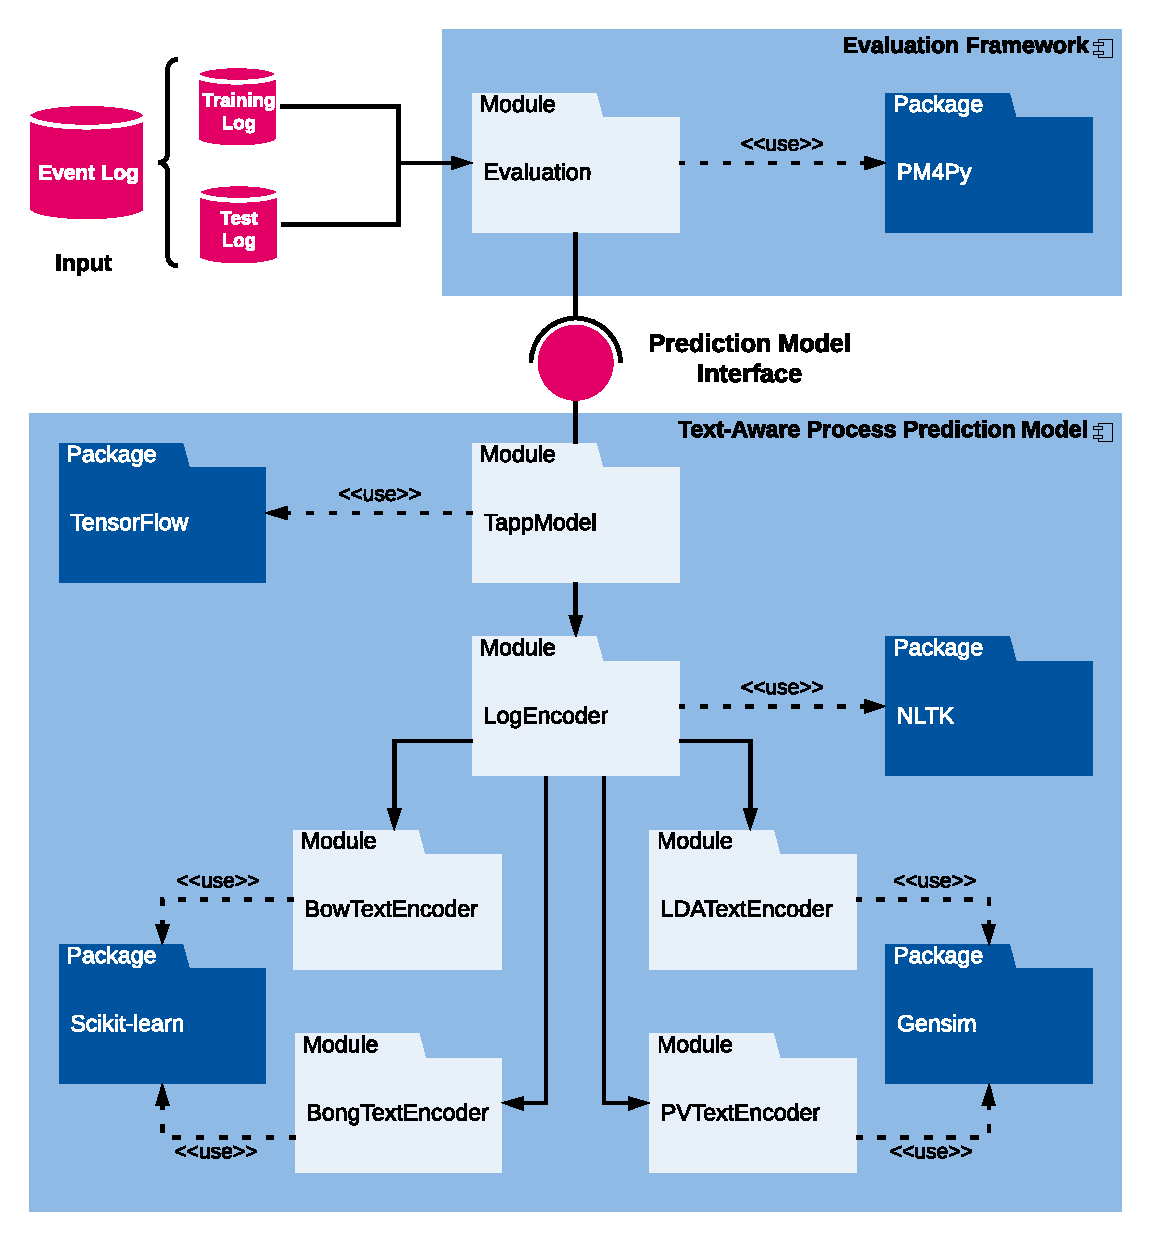
\includegraphics[width=\textwidth]{figures/implementation}
	\caption[Composition of the prediction model]{Modules and packages for the composition of the prediction model component.}
	\label{fig:/implementation}
\end{figure}